%%%%%%%%%%%%%%%%%%%%%%%%%%%%%%%%%%%%%%%%%
% University/School Laboratory Report
% LaTeX Template
% Version 3.1 (25/3/14)
%
% This template has been downloaded from:
% http://www.LaTeXTemplates.com
%
% Original author:
% Linux and Unix Users Group at Virginia Tech Wiki
% (https://vtluug.org/wiki/Example_LaTeX_chem_lab_report)
%
% License:
% CC BY-NC-SA 3.0 (http://creativecommons.org/licenses/by-nc-sa/3.0/)
%
%%%%%%%%%%%%%%%%%%%%%%%%%%%%%%%%%%%%%%%%%

%----------------------------------------------------------------------------------------
%	PACKAGES AND DOCUMENT CONFIGURATIONS
%----------------------------------------------------------------------------------------

\documentclass[a4paper,11pt]{scrartcl}

\usepackage[left=2.5cm, right=2.5cm]{geometry}

\usepackage[version=3]{mhchem} % Package for chemical equation typesetting
\usepackage{siunitx} % Provides the \SI{}{} and \si{} command for typesetting SI units
\usepackage{graphicx} % Required for the inclusion of images
\usepackage{natbib} % Required to change bibliography style to APA
%\usepackage[style=alphabetic]{biblatex}
\usepackage{amsfonts,amsmath,amssymb,amsthm,mathtools} % AMS Mathepakete
\usepackage{booktabs}
\usepackage[list=true, font=large, labelfont=bf,labelformat=brace, position=top]{subcaption}
\usepackage{blindtext}
\usepackage{caption} % um captions anzupassen und Subfigures aus LOF auszuschließen
%\usepackage[ngerman]{babel} % Paket um Deutsch als Sprache festzulegen
\usepackage{float}
\usepackage{tcolorbox}
\usepackage{tikz} % used for the schematic of the labeling errors
\usetikzlibrary{positioning}
\usepackage{hyperref}

\setcounter{tocdepth}{2}

%\addbibresource{sample.bib}

%\setlength\parindent{0pt} % Removes all indentation from paragraphs

\renewcommand{\labelenumi}{\alph{enumi}.} % Make numbering in the enumerate environment by letter rather than number (e.g. section 6)

\theoremstyle{definition}
\newtheorem{definition}{Definition}[section]

\newtheorem{variant}{Methodology}[section]

\captionsetup[subfigure]{list=no}

%\usepackage{times} % Uncomment to use the Times New Roman font

%----------------------------------------------------------------------------------------
%	DOCUMENT INFORMATION
%----------------------------------------------------------------------------------------

\title{Analysing the Impact of Label Noise\\on Training Neural Networks} % Title
\subtitle{M.Sc. Bioinformatics}

\author{Fabian \textsc{Fliedner}} % Author name

\date{\today} % Date for the report

\begin{document}
\maketitle % Insert the title, author and date
\begin{center}
\begin{tabular}{l r r}
Time of the Internship: & 08/2020 -- 10/2020& \\ % Date the experiment was performed
Instructor: & Dr. Nadine Flinner & Prof. Dr. Enrico Schleiff % Instructor/supervisor
\end{tabular}
\end{center}
\newpage
\tableofcontents
\listoffigures
\listoftables
\newpage

% If you wish to include an abstract, uncomment the lines below
\begin{abstract}
	% Abstract text
%	Deutsch und Stichpunkte:
%	\begin{itemize}
%		\item verwenden von Machine Learning (ML) für medizinische Anwendung.
%		\item Beispiel Nadines Arbeit - Analyse von Magenkarzinomen
%		\item Schwierigkeit dabei: Labels für molekulare Subklassen werden aus Sequenzdaten bezogen - nur ein Label pro Gewebeschnitt (oder pro Patient? -- Nadine fragen)
%		\item Praktikum: Analysiere die Auswirkungen von falsch gelabelten Trainingsdaten auf das Training
%		\item Results zusammenfassen
%	\end{itemize}
	Machine learning as an analytic tool is used in multiple disciplines and fields.
	%Von Spielen wie GO \cite{wu2007scalable} über Anwendungen in der Finanzwelt \cite{dixon2020machine} und ebenfalls in der Medizin \cite{deo2015machine}.
	From playing games to applications in the financial world and medicine.
	%Dabei wurden ML Ansätze bereits für die Klassifizierung von Brustkrebs verwendet \cite{amrane2018breast}.
	One of the medical applications is detection and classification of different cancer (sub-)types like breast cancer.
	%In diesem Praktikum untersuchen wir, in Hinblick auf die Klassifizierung von Magenkarzinomen mithilfe von ML, wie sich falsche oder unvollständige Datenlabels auf die Qualität des Trainings und die Fehlerraten auswirken.
	In this lab, we investigate how incorrect or incomplete data labels affect the quality of training and classification of a neural network, with respect to the analysis of gastric cancer.
	This study used training and mislabeling images of animals obtained from the ImageNet database as a proof of concept, which in further studies can be expanded and tested on medical image data.
	We could show, that training with larger datasets could improve the classification of the neural network and more reliably classify images with the wrong labels.
\end{abstract}

%----------------------------------------------------------------------------------------
%	SECTION 1
%----------------------------------------------------------------------------------------
\section{Introduction}
\begin{figure}[h]
	\centering
	\begin{center}
		\includegraphics[width=.9\textwidth]{Image_Intro/PastedGraphic-2.pdf}% Include the image placeholder.png
		\caption[Annotated gastric cancer tissue section]{Tissue section of gastric cancer tissue. Annotations for the different molecular subtypes.}%Magenkarzinom - Nadines Arbeit - Markierungen für verschiedene molekulare Subklassen}%TODO: genauere Beschreibung
		\label{fig:magenkarzinom_nadine}
	\end{center}
\end{figure}
%\cite{deng2009imagenet}

Machine learning as an analytical tool has various fields in which it can be implemented.
From applications in games such as chess \cite{lai2015giraffe} and Go (AlphaGo) \cite{wu2007scalable}, to analyses in the financial world \cite{dixon2020machine}, as well as in medicine \cite{deo2015machine}, e.g. for the classification of cancer types on the basis of tissue sections \cite{amrane2018breast}.

The group of Dr. Nadine Flinner (?) focuses on the use of computer vision to identify and classify gastric cancer.
Gastric cancer cases are divided into multiple molecular subtypes \cite{bass2014comprehensive}: Epstein–Barr virus (\emph{EBV})-positive, microsatellite instability (\emph{MSI}), genomically stable (\emph{GS}) and chromosomal instability (\emph{CIN}).

For training a neural network to classify these subtypes, tissue sections are assigned labels corresponding to the subtype obtained from genomic data.
However, cancer tissue is not homogeneous \cite{de1989gastric} (see \autoref{fig:magenkarzinom_nadine}), so tissue sections may contain areas where the label does not match the molecular subtype.

This lab is focused on an analysis of the impact of mislabeled datasets on the training of a neural network.
For this purpose, instead of medical data, images of animals from the ImageNet database \cite{deng2009imagenet} are used, since a neural network can be trained quickly on the basis of the different features.
%Allgemeines Statement: Verwendung von Machine Learning und Deep Learning in den letzten jahren gestiegen (?) %TODO: statistiken suchen
%Verwendung von ML (im genaueren Computer Vision) für Medizinische Anwendung und Untersuchung von Gewebeschnitten mit fokus auf Cancer- vs. Non-Cancer Analysen.
%Nadine Flinner arbeitet an der Analyse von Magenkarzinomen - verschiedene molekulare Subklassen (4 Stück: EBV, MSI, GS, CIN) mit dem Ansatz Machine Learning zu verwenden, um die verschiedenen Subklassen zu unterscheiden.
%Dieses Praktikum beschäftigt sich mit der Analyse von Effekten, die Fehler im Labeling von Trainingsdaten auf das Training eines Neural Networks haben.

\subsection{Definitions}
\label{definitions}
\begin{definition}[Observable Error]\label{def:observableerror}
	The error calculated by the neural network, comparing the prediction made for an image of the validation set with the label with which the neural network was trained (containing purposefully mislabeled images).
	This describes the error rates which can be directly observed and calculated by the neural network.
\end{definition}
\begin{definition}[True Error]\label{def:trueerror}
	A second error calculated by comparing the prediction made by the neural network to the true label of the images in the validation set (which is known beforehand).
	This error can't be obtained in real data.
	It has to be calculated by purposefully introducing errors into the data-sets and comparing the prediction of the neural network with the label assigned to the data and the true label, which is hidden from the network.
\end{definition}

%die Definitionen kann man auch referenzieren über \ref{def:observableerror} und \ref{def:trueerror}
%----------------------------------------------------------------------------------------
%	SECTION 2
%----------------------------------------------------------------------------------------

\section{Materials and Method}
\subsection{ImageNet data}
To train the neural network and have a sizeable amount of images for each of the classes, we used pictures of \emph{dogs}, \emph{cats} and later \emph{mice} and small \emph{birds}, downloaded from the ImageNet database.
\begin{tcolorbox}[colback=red!5,colframe=red!40!black,title=Disclaimer regarding validation and test data]
	While ideally the test data would be fully independent from the training and validation data, in this study all of the images were obtained from ImageNet and split into the three groups prior to training the network.
\end{tcolorbox}\label{test}
%While ideally the test data would be fully independent from the training and validation data, in this study all of the images were obtained from ImageNet and split into the three groups prior to training the network.
\subsection[Data-frame creation]{Creation of dataframes and introduction of labeling errors}
A Python script is used to generate a dataframe for the training of the neural network.
The dataframe contains information about the filenames and two different labels.
One is the label used in training the neural network (called 'label') while the other (called 'true\_label') is used for the "manual" calculation of the \emph{True Error}.
The true label is obtained through the filename (ImageNet provides a document which can be used to map the filenames to a human readable label), while the label used in training the network is 'randomly' assigned.
Following these labels are five columns containing information if the image is used in training or validation of the neural network.
Each image is used four times in training and once for the validation [five-fold cross-validation].
An example is shown in \autoref{tab:example_dataframe}. %.. an example is shown below
A schematic for the introduction of labeling errors is shown in \autoref{img:schematics}.

\begin{table}[h]% Add the following just after the closing bracket on this line to specify a position for the table on the page: [h], [t], [b] or [p] - these mean: here, top, bottom and on a separate page, respectively
\centering % Centres the table on the page, comment out to left-justify
\begin{tabular}{c c c c}
%\cmidrule(l){2-6}
file&label&true\_label&validation [0-4]\\
% Column names row valid\_3
\midrule % In-table horizontal line
\texttt{Filename.jpg} & \texttt{label\_a} & \texttt{label\_b} & \texttt{True/False}\\
\vdots&&&\\
\end{tabular}
\caption[Example Dataframe]{An example for the used dataframes. Validation [0-4] combines five columns used for the five-fold cross-validation} % Table caption, can be commented out if no caption is required
\label{tab:example_dataframe} % A label for referencing this table elsewhere, references are used in text as \autoref{label}
\end{table}

\begin{figure}[h!]%tbp]
	\centering
	\begin{subfigure}[t]{0.32\textwidth}
		\centering
		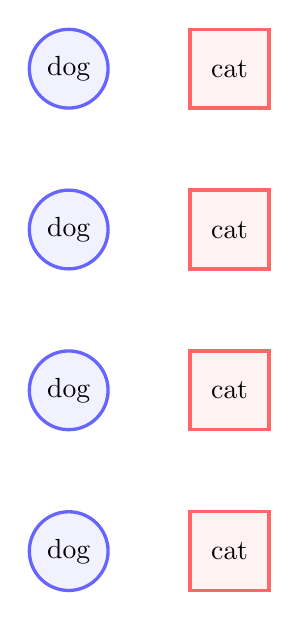
\begin{tikzpicture}[
			dognode/.style={circle, draw=blue!60, fill=blue!5, very thick, minimum size=10mm},
			catnode/.style={rectangle, draw=red!60, fill=red!5, very thick, minimum size=10mm},
			]
			%Nodes
			\node[dognode] (dog1) 					{dog};
			\node[dognode] (dog2)	[below=of dog1] {dog};
			\node[dognode] (dog3)   [below=of dog2] {dog};
			\node[dognode] (dog4)   [below=of dog3] {dog};

			\node[catnode] (cat1) 	[right=of dog1] {cat};
			\node[catnode] (cat2)   [right=of dog2] {cat};
			\node[catnode] (cat3)   [right=of dog3] {cat};
			\node[catnode] (cat4)   [right=of dog4] {cat};
		\end{tikzpicture}\vspace{5mm}
		\subcaption{Training without any \\labeling errors.}
		\label{img:schematic_noError}
	\end{subfigure}
	\begin{subfigure}[t]{0.32\textwidth}
		\centering
		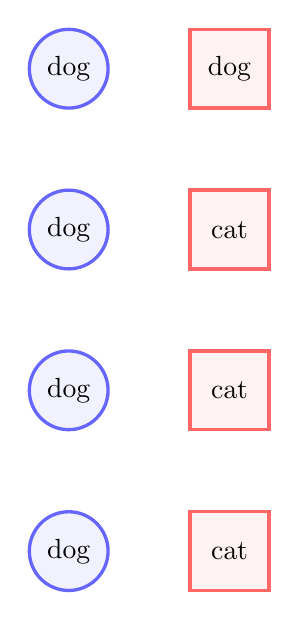
\begin{tikzpicture}[
			dognode/.style={circle, draw=blue!60, fill=blue!5, very thick, minimum size=10mm},
			catnode/.style={rectangle, draw=red!60, fill=red!5, very thick, minimum size=10mm},
			]
			%Nodes
			\node[dognode] (dog1) 					{dog};
			\node[dognode] (dog2)	[below=of dog1] {dog};
			\node[dognode] (dog3)   [below=of dog2] {dog};
			\node[dognode] (dog4)   [below=of dog3] {dog};

			\node[catnode] (cat1) 	[right=of dog1] {dog};
			\node[catnode] (cat2)   [right=of dog2] {cat};
			\node[catnode] (cat3)   [right=of dog3] {cat};
			\node[catnode] (cat4)   [right=of dog4] {cat};
		\end{tikzpicture}\vspace{5mm}
		\subcaption{Training with an image showing a dog falsely\\ labeled as a cat.}
		\label{img:schematic_asymetrical}
	\end{subfigure}
	\begin{subfigure}[t]{0.32\textwidth}
		\centering
		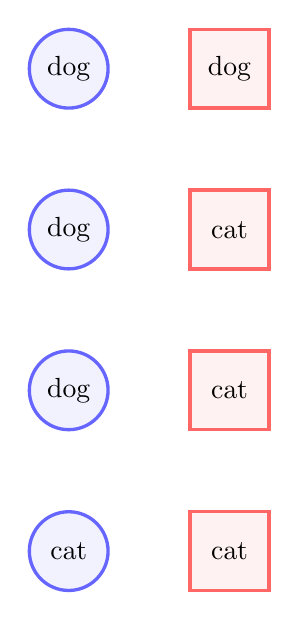
\begin{tikzpicture}[
			dognode/.style={circle, draw=blue!60, fill=blue!5, very thick, minimum size=10mm},
			catnode/.style={rectangle, draw=red!60, fill=red!5, very thick, minimum size=10mm},
			]
			%Nodes
			\node[dognode] (dog1) 					{dog};
			\node[dognode] (dog2)	[below=of dog1] {dog};
			\node[dognode] (dog3)   [below=of dog2] {dog};
			\node[dognode] (dog4)   [below=of dog3] {cat};

			\node[catnode] (cat1) 	[right=of dog1] {dog};
			\node[catnode] (cat2)   [right=of dog2] {cat};
			\node[catnode] (cat3)   [right=of dog3] {cat};
			\node[catnode] (cat4)   [right=of dog4] {cat};
		\end{tikzpicture}\vspace{5mm}
		\subcaption{Training with labeling\\ errors in both subclasses.}
		\label{img:schematic_symmetrical}
	\end{subfigure}
	\caption[Labeling schematic]{Schematic of how the labeling errors are introduced. Blue circles are images showing dogs, red squares are images of cats, with the label corresponding to the label used for training the network.}
	\label{img:schematics}
\end{figure}
\subsection{Training the network}
Using the dataframes we trained multiple neural networks with different starting conditions. One of the variables was the amount of data used. We started with a low number of images, to quickly obtain a base line on which we could calculate the different errors. We then increased the amount of data used for training and validation by a factor of $10$ and $100$ in comparison to our first runs. Another variation was the number of classes, as well as how the labeling errors are introduced into the data.

%----------------------------------------------------------------------------------------
%	SECTION 3
%----------------------------------------------------------------------------------------

\section{Results}
In all of the tests (studies?) we could observe increasing error rates with higher amounts of data containing labeling errors
\subsection[Two labels, labeling errors in one class]{Training a network with two classes with labeling errors in one of the classes.}
\begin{figure}[!h]
\centering
%\begin{center}
\includegraphics[width=.8\textwidth]{Plots_1/0300_full_comparison_noTitle.pdf}% Include the image placeholder.png
\caption[Error rates for training with two classes]{Comparing the development of different error types for training with 300 images in each of the two classes. Labeling errors only occurring in one of the classes.}
\label{fig:two_class_full_300}
%\end{center}
\end{figure}
When introducing the labeling error into one of the classes (in this case having images of \emph{cats} labeled as \emph{dogs}, shown schematically in \ref{img:schematic_asymetrical}) we noticed a higher \emph{observable error} compared to the \emph{true error} in both validation and testing dataset for percentage of labeling errors $\geq0\%$, as shown in \autoref{fig:two_class_full_300}.
At $0\%$ labeling error every image the network evaluates as incorrect is correctly identified as incorrect, since all of the assigned labels are the true labels.
Another observation is, that error rates calculated from the test dataset is slightly higher than the ones calculated from the validation dataset.
% This can be explained (?) by the tendency of the network to optimize the error rates for the validation datasets.
When comparing the error rates for different amounts of data-points (see \autoref{fig:development_30_300_3000}) it shows a lower error rates (both \emph{observable} and \emph{true error}) for higher amounts of images.
Looking at the combined confusion matrices in \autoref{fig:onesided_confusion_matrix} (specifically \ref{subfig:confusion_25_00} \& \ref{subfig:confusion_50_00}) over all runs a majority of the images ($>90\%$) with an incorrect label are predicted correctly, according to the true label.
while this cannot be observed directly, it shows that in our dataset the network can still reliably match the test images even with labeling errors that have a significant proportion (25\%) of the training dataset.

%\begin{itemize}
%    \item observable error is always higher than the true error (except for 0\% mislabel, where True == Observable) $\rightarrow$ not surprising, since the neural network evaluates a prediction as incorrect if the prediction is equal to the true label of mislabeled data
%    \item Test error is slightly higher than validation error $\rightarrow$ ideally test data is completely independent of the training- and validation data-set. Training optimizes for validation data.
%\end{itemize}
\begin{figure}[!h]%tbp]
	\centering
\begin{subfigure}[t]{0.49\textwidth}
\includegraphics[width=0.99\textwidth]{Plots_1/ObservableTest_extreme_comparison_noTitle.pdf}
\subcaption{Observable error}
\end{subfigure}
\begin{subfigure}[t]{0.49\textwidth}
\includegraphics[width=0.99\textwidth]{Plots_1/TrueTest_extreme_comparison_noTitle.pdf}
\subcaption{True error}
\end{subfigure}
\caption[Error development for different training sizes]{Comparing the observable and true error rates for training with different amounts of data.}
\label{fig:development_30_300_3000}
\end{figure}

\begin{figure}[!h]%tbp]
	\centering
\centering
\begin{subfigure}[t]{0.32\textwidth}
\includegraphics[width=0.99\textwidth]{Plots_1/compound_3000_00_00_no_Title.pdf}
\subcaption{no mislabeled training data}
\end{subfigure}
\begin{subfigure}[t]{0.32\textwidth}
\includegraphics[width=0.99\textwidth]{Plots_1/compound_3000_25_00_no_Title.pdf}
\subcaption{25\% of cats are labeled as dogs}
\label{subfig:confusion_25_00}
\end{subfigure}
\begin{subfigure}[t]{0.32\textwidth}
\includegraphics[width=0.99\textwidth]{Plots_1/compound_3000_50_00_no_Title.pdf}
\subcaption{50\% of cats are labeled as dogs}
\label{subfig:confusion_50_00}
\end{subfigure}
\caption[Confusion matrices for labeling errors in one class.]{Confusion matrices for training with labeling errors occurring in one of the two classes.}
\label{fig:onesided_confusion_matrix}
\end{figure}

%\subsubsection{Conclusion for these Plots}
%\begin{itemize}
%    \item More images with false labels $\rightarrow$ higher error rates
%    \item Higher number of images in training $\rightarrow$ effect of falsely labeled data can be mitigated\\(can't actually be observed)
%    \item  %\autoref{fig:onesided_confusion_matrix}
%\end{itemize}

\subsection[Two labels, labeling errors in both classes]{Training a network with two classes with labeling errors in both classes.}
In this setup we introduced the labeling errors into both classes the network is training with, as schematically shown in \autoref{img:schematic_symmetrical}.
Even with the introduction of a labeling error of 50\% in one class and 20\% in another, the true error is less than 15\% \autoref{subfig:confusion_20_20} and \ref{subfig:confusion_20_50}.
With labeling errors in both classes of 40-50\%, the network's predictions become a coin flip, as reflected in \autoref{subfig:confusion_50_50}.
\autoref{fig:cross_mislabel_heatmaps} shows that the effect of the labeling errors is symmetrical with both classes.
There is a noticeable difference in the development of the observable versus true error.
While the observable error behaves almost linearly, the effect of the labeling errors on the true error is very low until the percentage of labeling errors approaches 50\%.
\autoref{subfig:cross_mislabel_difference_heatmap} shows the differences between observable and true error.
Since for no labeling errors both describe the same error, the difference is 0, which is also the case for 50\% labeling errors in both classes, where the network has the exact same amount of images showing cats being labeled as dogs and vice versa.
\begin{figure}[H]
\centering
\begin{subfigure}[t]{0.32\textwidth}
\includegraphics[width=0.99\textwidth]{Plots_2/compound_3000_20_20_no_Title_same_scale.pdf}
\subcaption{20\% of each class labeled as the other}
\label{subfig:confusion_20_20}
\end{subfigure}
\begin{subfigure}[t]{0.32\textwidth}
\includegraphics[width=0.99\textwidth]{Plots_2/compound_3000_20_50_no_Title_same_scale.pdf}
\subcaption{20\% of cats labeled as dogs, 50\% of dogs labeled as cats}
\label{subfig:confusion_20_50}
\end{subfigure}
\begin{subfigure}[t]{0.32\textwidth}
\includegraphics[width=0.99\textwidth]{Plots_2/compound_3000_50_50_no_Title_same_scale.pdf}
\subcaption{50\% of each class labeled as the other}
\label{subfig:confusion_50_50}
\end{subfigure}
\caption[Confusion matrices for labeling errors in both classes.]{Confusion matrices for training with labeling errors occurring in both classes.}
\label{fig:crossed_confusion_matrix}
\end{figure}

\begin{figure}%[htbp]
\centering
\begin{subfigure}[t]{0.32\textwidth}
\includegraphics[width=0.97\textwidth]{Plots_2/3000_otest_images_new.pdf}
\subcaption{Development of the observable error for differing amounts of labeling errors in both classes.}
\label{subfig:cross_mislabel_observable}
\end{subfigure}
\begin{subfigure}[t]{0.32\textwidth}
\includegraphics[width=0.97\textwidth]{Plots_2/3000_ttest_images_new.pdf}
\subcaption{Development of the true error for differing amounts of labeling errors in both classes.}
\label{subfig:cross_mislabel_true}
\end{subfigure}
\begin{subfigure}[t]{0.32\textwidth}
\includegraphics[width=0.97\textwidth]{Plots_2/3000_difference_images_new.pdf}
\subcaption{difference between the observable and true error.~}
\label{subfig:cross_mislabel_difference_heatmap}
\end{subfigure}
\caption[Heatmaps comparing error rates in training with labeling errors in both classes.]{Comparing the development of the observable and true error when labeling errors occur in both of the classes.}
\label{fig:cross_mislabel_heatmaps}
\end{figure}

%\subsubsection{Conclusions for asymmetric mislabeling with two classes}
%
%\begin{itemize}
%    \item While only 20\% of each label is falsely labeled \autoref{subfig:confusion_20_20} or imbalanced \autoref{subfig:confusion_20_50} the predictions which are observed as being incorrect would still largely predict the correct labels (90\%/80\%)
%    \item If both labels contain 50\% of falsely labeled data the predictions turn into a coin flip, which can also be observed in \autoref{subfig:confusion_50_50}
%    \item \autoref{fig:cross_mislabel_heatmaps} shows that falsely labeling from one to the other behaves basically symmetrically.
%    \item \autoref{subfig:cross_mislabel_difference_heatmap} shows the difference between the observable error and the true error. with 50\% mislabeled data both errors are $\approx$50\% so the difference is 0, for no mislabeled data the observable error is equal to the true error.
%\end{itemize}

\subsection[Four labels, one class evenly distributed in all others]{Training a network with four classes. One class mislabeled and evenly distributed.}
%\begin{itemize}
%    \item Introducing two new classes: \textbf{Birds} and \textbf{Mice}.
%    \item Labeling a percentage of cats as all of the different labels (at the end each of the other labels composes of 50\% cats)
%    \item Mislabeling symmetrically $\rightarrow$ always the same \% of cats in the other labels.
%\end{itemize}
For this study we added two additional classes \emph{birds} and \emph{mice}.
We introduced labeling error occurs symmetrically into all of the non-\emph{cat}-classes, which means for every class of images not showing cats we added a percentage of images showing cats with the label of the class.

\begin{figure}%[htbp]
\centering
%\begin{subfigure}[t]{0.8\textwidth}
\includegraphics[width=0.8\textwidth]{Plots_3/3_Full_comparison_symmetric_mislabel_4_classes.pdf}
\caption[Development of the error rates]{Comparing the development of different error types for training with 300 images in each of the four classes. Labeling errors are introduced by having images of cats among all of the other classes.}
\label{fig:four_classes_full_comparison}
%\end{subfigure}
\end{figure}

\begin{figure}%[htbp]
\centering
\begin{subfigure}[t]{0.49\textwidth}
\includegraphics[width=0.99\textwidth]{Plots_3/Observable_Test_Error_comparison.pdf}
\subcaption{Development of the observable error with different amounts of images}
\label{subfig:four_classes_observable_error}
\end{subfigure}
\begin{subfigure}[t]{0.49\textwidth}
\includegraphics[width=0.99\textwidth]{Plots_3/True_Test_Error_comparison.pdf}
\subcaption{Development of the true error with\\different amounts of images}
\label{subfig:four_classes_true_error}
\end{subfigure}
\caption[Error development for different training sizes]{Comparing the observable and true error rates for training with different amounts of data. Labeling errors of up to 50\% occurring in three of four labels.}
\label{fig:four_class_error_development}
\end{figure}

%\subsubsection{Conclusions for symmetric mislabeling with four classes}
%\begin{itemize}
%    %\item \autoref{fig:four_classes_full_comparison} shows a similar development as \autoref{fig:two_class_full_300}:\\
%    %test error is slightly higher than validation error, observable error is significantly higher than true error.
%    %\item similar to the previous point the error development for different amounts of training data behaves similarly to the case with two different classes. (Anm.: \textsc{für den Fall 40 $\rightarrow$ 200 ist der True Error für mehr falsche Labels höher - vsl. begründet durch 25 Runs (5-Fold Crossvalidation, 5 Runs))}
%    \item \textbf{CONCLUSIONS:} while the development for an increased number of classes behaves like the equivalent case with two classes, the absolute error is higher.\\Examples:
%    \subitem four classes: 50\% mislabel 1000 Images/Label $\rightarrow\approx25\%$ True error
%    \subitem two classes: 50\% mislabel 300 Images/Label $\rightarrow\approx25\%$ True error
%    \item \textbf{CONCLUSIONS:} can still mitigate the effect of the false labels by training the neural network with more data
%\end{itemize}
Comparing the development of the error rates with four classes \autoref{fig:four_classes_full_comparison} to the study with only two classes \autoref{fig:two_class_full_300} shows similar trends, with the observable error rates being significantly higher than the true error and the error rates calculated from the validation dataset slightly lower than the ones obtained from the test datasets.
The conclusion that we can mitigate labeling errors by increasing the amount of data used for training the neural network, with the higher true error in the run with 200 images per label (\autoref{subfig:four_classes_true_error}) can be explained through the limited amount of repetitions.

\subsection[Two labels, introduction of an unknown third class]{Training a network with two known classes and introducing a hidden/unknown third class.}
%\begin{itemize}
%    \item Added images of birds into both data-sets.
%    \item Different amounts in each data-set possible.
%    \item Changed the computation of the true error slightly:\\
%    since the hidden subclass can't be predicted at all, the true error is calculated by ignoring the predictions for the hidden subclass.
%    \item Bias in fig~\autoref{subfig:confusion_25_25_hidden} (Birds towards dogs) is result of combining all 25 Confusion Matrices.\\
%    Not consistent through all runs/crossvalidations % ToDo: Beispiele für beide Varianten einfügen
%\end{itemize}
%Für diese Untersuchung wurden Bilder von Vögeln (in diesem Fall vor allem von Meisen und ähnlichen Kleinvögeln) in die Trainingsdatensätze als Hunde sowie Katzen eingefügt.
For this study, images of birds were inserted into the training datasets as dogs as well as cats.
%Die Menge der eingefügten, falsch gelabelten Bilder, wurde in fünf Prozent Schritten bis zu 25\% erhöht und konnte unterschiedlich für die beiden detektierbaren Klassen sein.
The amount of inserted mislabeled images, was increased in five percent increments up to 25\% and could be different for the two classes.
%Da die versteckte Klasse 'Vögel' von dem Neural Network nicht erkannt werden kann (das Netzwerk trainiert weiterhin nur auf zwei verschiedene Klassen), haben wir die Berechnung des 'True Error' nur auf den Fehlerraten der beiden Klassen durchgeführt, auf die das Neural Network trainiert.
Since the hidden class \emph{birds} cannot be detected by the Neural Network, we adjusted the definition of the \emph{true error}.
Because the network continues to train on the two classes \emph{cats} and \emph{dogs} all images of birds assigned to either class would count towards the True Error.
This would result in the True Error being equal to the number of images inserted.
%In diesem Datensatz wurde die Definition \autoref{def:trueerror} angepasst, da das Netzwerk weiterhin nur auf zwei Klassen trainiert (Hunde und Katzen) und somit alle Bilder von Vögeln, die einer der beiden Klassen zugeordnet werden, als True Error gewertet würden.
%Dies führt dazu, dass der True Error gleich der Anzahl an eingefügten Bildern ist.
%Aus diesem Grund wird der True Error nur für Bilder berechnet, die nicht Teil der hidden subclass sind.
For this reason, we calculate the True Error only for images that are not part of the hidden subclass.\textbf{}

\begin{figure}[htbp]
\centering
\begin{subfigure}[t]{0.49\textwidth}
\includegraphics[width=0.99\textwidth]{Plots_4/compound_1000_10_00_no_Title_same_scale_hidden.pdf}
\subcaption{10\% of the images labeled as cats are showing birds}
\label{subfig:confusion_10_00_hidden}
\end{subfigure}
\begin{subfigure}[t]{0.49\textwidth}
\includegraphics[width=0.99\textwidth]{Plots_4/compound_1000_25_25_no_Title_same_scale_hidden.pdf}
\subcaption{25\% of the images in both classes are showing birds, labeled as either dogs or cats.}
\label{subfig:confusion_25_25_hidden}
\end{subfigure}
\caption[Confusion matrix hidden class.]{Confusion matrices for a hidden class which is spread between the other classes.}
\label{fig:confusion_matrix_hidden}
\end{figure}

\begin{table}[H]% Add the following just after the closing bracket on this line to specify a position for the table on the page: [h], [t], [b] or [p] - these mean: here, top, bottom and on a separate page, respectively
	\centering % Centres the table on the page, comment out to left-justify
	\begin{tabular}{ c c | r r | r r | r r | r r } % The final bracket specifies the number of columns in the table along with left and right borders which are specified using vertical pipes (|); each column can be left, right or center-justified using l, r or c. Columns will widen to hold the content in them by default, to specify a precise width, use p{width}, e.g. p{5cm}
		\toprule % Top horizontal line
		\multicolumn{2}{c}{\textbf{label}} & \multicolumn{8}{c}{\textbf{predictions}} \\ % Amalgamating several columns into one cell is done using the \multicolumn command with the number of columns to amalgamate as the first argument and then the justification (l, r or c)
		%\cmidrule(l){2-6} % Horizontal line spanning less than the full width of the table - you can add (r) or (l) just before the opening curly bracket to shorten the rule on the left or right side
		\textbf{train}  & \textbf{true} &cat&dog&cat&dog&cat&dog&cat&dog\\
		% Column names row valid\_3
		\midrule % In-table horizontal line
		cat & cat& 145 & 6 & 140 & 4 & 152 & 1 & 138 & 7 \\
		dog & dog  & 3 & 147 & 5 & 141 & 4 & 142 & 2 & 140 \\
		dog & bird  & 33 & 17 & 24 & 30 & 25 & 29 & 28 & 30 \\
		cat & bird  & 33 & 17 & 21 & 35 & 30 & 17 & 25 & 30\\
		%n02123159\_2586.JPEG & cat & cat & False & $\cdots$ & False &\\
		%\midrule % In-table horizontal line
		%\midrule % In-table horizontal line
		%Average Rate & 0.920 & 0.882 & 0.477 & 0.539 & 0.923\\ % Summary/total row
		\midrule
		 & & \multicolumn{2}{c|}{\textbf{run 3}}& \multicolumn{2}{c|}{\textbf{run 6}}& \multicolumn{2}{c|}{\textbf{run 12}}& \multicolumn{2}{c}{\textbf{run 21}}\\
		\bottomrule % Bottom horizontal line

	\end{tabular}
	\caption[Excerpt of confusion matrices]{excerpt of confusion matrices from different runs, with 25\% of both labels being mislabeled birds} % Table caption, can be commented out if no caption is required

	\label{tab:examples_against_bias} % A label for referencing this table elsewhere, references are used in text as \autoref{label}
\end{table}


\begin{figure}%[htbp]
\centering
\begin{subfigure}[t]{0.49\textwidth}
\includegraphics[width=0.99\textwidth]{Plots_4/1000_ovalid_images_hidden.pdf}
\subcaption{Observable error development}
\label{subfig:observable_heatmap_hidden}
\end{subfigure}
\begin{subfigure}[t]{0.49\textwidth}
\includegraphics[width=0.99\textwidth]{Plots_4/1000_tvalid_images_hidden.pdf}
\subcaption{True error development}
\label{subfig:tue_heatmap_hidden}
\end{subfigure}
\caption[Heatmaps comparing error rates when introducing a hidden class.]{Comparing the development of the observable and true error when introducing a hidden subclass into one or both classes.}
\label{fig:heatmaps_hidden}
\end{figure}

\subsubsection{Conclusions for training with a hidden subclass}
%\begin{itemize}
%    \item The influence of a hidden subclass on the true error doesn't exist, since (in our case) cats and dogs are distinct enough from each other (and from birds).
%    \item the observable error doesn't chance much if the subclass is only spread in one of both training data-sets, since most of the images are predicted to be the trained label (\autoref{subfig:confusion_10_00_hidden}: only five birds in 25 runs are predicted to be dogs, after being trained to be cats)
%    \item for an equal split (25\% of both labels are actually the hidden class) the training results in a coin flip, for the number of runs the data shows a slight bias towards predicting birds as dogs.
%\end{itemize}
Since we changed the calculation of the true error for this analysis, the effect of introducing a hidden class is nonexistant, since all of the analyzed classes are very distinct from each other.

The effect on the observable error depends on how the unknown subclass is spread throughout the training and validation data-sets.
If the subclass is mostly contained in one of the trained subclasses the observable doesn't change significantly compared to a network trained only on two classes, since most of the images are predicted to be of the label they are wrongly associated with (see \autoref{subfig:confusion_10_00_hidden}, only 1\% of the images containing birds, labeled as cats were predicted to be dogs).
This is also reflected in \autoref{fig:heatmaps_hidden}, showing a homogenous distribution of the true error, regardless of the amount of images showing birds added to both classes.

When the hidden subclass is spread more or less equally between the other two labels it turns into a coin flip which label is assigned to images of birds.
While \autoref{subfig:confusion_25_25_hidden} shows a slight bias towards dogs, this seems to be a product of adding up all of the runs. Looking at \autoref{tab:examples_against_bias} also shows examples, where the Network has a bias towards predicting birds as cats.

\subsection[Comparison of different amounts of data]{Comparing the development of the error rates in dependance of training size}
\begin{figure}[htbp]
\centering
\includegraphics[width=0.8\textwidth]{Plots_5/Error_Evolution_hidden_vs_mislabeled.pdf}
\caption[Comparison between hidden class and labeling errors.]{Comparing the change of the observable error between the runs with a hidden subclass and labeling errors in both classes, when training with different amounts of data.}
\label{fig:compare_hidden_vs_mislabel}
\end{figure}
%\subsubsection{Conclusion for the comparison of both labeling errors}
%\begin{itemize}
%    \item the absolute error is higher for mislabeled data.
%    \item only 25 runs on one data-set overall $\rightarrow$ not enough data to draw significant conclusions.
%    \item Slope seems to be the same, so only using this data you couldn't distinguish which type of labeling error is in the data
%\end{itemize}


%----------------------------------------------------------------------------------------
%	SECTION 5
%----------------------------------------------------------------------------------------
Unsurprisingly, if the data contains more labeling errors, the error rates (true and especially observable) of the predictions increase.
Comparing the true errors for the validation data-set with an increasing number of images, we see a decrease in the true error rate for a similar percentage of labeling errors -- with an exception for a high percentages of mislabeled data (50\% mislabeled cats $\equiv$ 25\% of overall Data mislabeled) \autoref{fig:development_30_300_3000} and \autoref{fig:four_class_error_development}.
The difference, however, is within one standard deviation, so we can attribute this to a small number of 25 runs, five runs with a five-fold cross-validation each.

Comparing this figure, where the amount of data increases by an order of magnitude in between runs, to the previous one, the error rate between the different runs decreases significantly. This leads to the assumption that we can mitigate the effect of false labels in training data by increasing the amount of data used in training significantly (10$\times$/100$\times$).
%\section{Conclusions}
%\subsection{Hidden subclass}
%\section{Discussion}
%\subsection{deutsch und stichpunktartig}
%Diskussion Praktikum
%\begin{itemize}
%\item Daten zeigen (möglicherweise) Trend an dem sich erkennen lässt, dass etwas mit den Daten nicht stimmt (Stand 13/10/2020 - zusätzlichen Plot).
%\item Über die beobachtbare Fehlerrate (observable Error) lässt sich feststellen, ob eine zusätzliche bisher unbekannte Subklasse in den Daten vorliegt, sofern diese annähernd gleichverteilt in den anderen Daten ist.
%\item Liegen falsche Label in den Daten vor, so nimmt die Fehlerrate im asymmetrischen Fall (einseitig falsch gelabelt nur a$\rightarrow$b)
%\end{itemize}

%Die Daten zeigen, dass man anhand einer Trainingsreihe mit unterschiedlichen


\section{Discussion and Outlook}
%As a follow-up for this study it can be explored if the effect of falsely labeled training data can be detected during (or at least after) training the NN - either through looking at the loss or by looking at the error rate/accuracy.
%Da in diesem Praktikum bisher nur auf ImageNet Daten gearbeitet wurde, ist der nächste logische Schritt, die Methode auf medizinische Bilder von Magenkarzinomen anzuwenden, um zu überprüfen, ob sich heterogenere Bilder ähnlich verhalten, wie die sehr distinkten Bilder, die in diesem Praktikum verwendet wurden. Die verwendeten ImageNet Daten und Klassen sind sehr distinkt und wurden von FastAI bereits verwendet, um die Neuralen Netze zu trainieren. Eine Betrachtung der Laufzeiten im Vergleich zu den aktuellen Daten liegt daher nah.
%Darüber hinaus kann man untersuchen, ob sich unterscheiden lässt, ob die Daten ein falsches Label tragen, oder sich in den Daten eine Klasse befindet, die vorher nicht bekannt war.
%In der aktuellen Studie wurde nur anhand der Fehlerrate verglichen, wie sich die Fehler auf das Training auswirken. Für die folgenden Analysen sollten weitere Kriterien (z.B. Loss) zum Vergleich herangezogen werden.
%Zudem kann man im Training betrachten, wie bestimmte Bilder in unterschiedlichen Runs predicted werden. So könnte man im Kontext dieses Praktikums betrachten, ob Bilder auf denen Katzen zu sehen sind, häufiger als per Zufall erwartet dem Label 'Katze' zugeordnet werden, unabhängig von dem Label, das ihnen zugeordnet ist.

Since this study has only worked with ImageNet data so far, the next logical step is to apply the method to medical images of gastric cancer to see if more heterogeneous images behave similarly to the very distinct ones used in this study. The ImageNet data and classes used are highly distinctive and have already been used by FastAI to train the neural networks.

In addition, it is possible to investigate whether can be detected if the data carries a wrong label or there is a class in the data that was not known before, either by looking at the loss or comparing the error-rates.

In the current study, only the error rate was used to compare how the errors affect the training. For subsequent analyses, other criteria (e.g. loss) should be used for further comparison.

In addition, it can be analyzed how certain images are predicted in different runs during training. For example, in the context of this lab, one could look at whether images that have cats on them are predicted as \emph{cats} more often than expected by chance, regardless of the assigned label.

\subsection{Ausblick/Vergleich mit Literatur}
The results of this lab are concurrent with the findings of \cite{rolnick_label_noise}. While the scope of this lab was much smaller, it still provided the same basic conclusions, that labeling noise can be mitigated with large enough datasets. We also used the worst possible conditions, where the label noise was not uniform over multiple labels, but rather just one label, so the only type of label noise was highly repetitive.



%----------------------------------------------------------------------------------------
%	BIBLIOGRAPHY
%----------------------------------------------------------------------------------------

\bibliographystyle{apalike}

\bibliography{label_noise}

%----------------------------------------------------------------------------------------


\end{document}